\documentclass[class=NTHU_thesis, crop=false]{standalone}
\begin{document}


\chapter{Introduction}
\label{chap:Introduction}
In the universe, the galaxies are observed to violate Newton's second law with the rotation of the observable matters which is faster than expected. Thus it is thought that there are invisible matters called Dark Matter (DM) generating additional gravity to accelerate the rotation. The most popular hypothesis is proposed that DM is a stable and electrically natural particle $\chi$ which only has weak and gravitational interaction with the Standard Model (SM) particles. Thanks to the characteristics, we can try to search such particle at the Large Hadron Collider (LHC).

One possible model of DM is a Type-II two-Higgs-doublet model (2HDM) with an additional U(1)$_{Z^\prime}$ gauge symmetry, known as the $Z^\prime$-2HDM model. A light scalar $h$, which is identified as the SM Higgs boson, and a pseudo-scalar $A$ are introduced among this model, together with a striking process shown in \cref{fig:DM-Model}. The process has the attribute targeted by the collider searches that the final state is DM following with a detectable particle, the SM Higgs boson $h$ in this case. Due to the single visible Higgs boson in the final state, the search for DM of $Z^\prime$-2HDM model is called the monoH analysis. This analysis exploits the largest decay branching ratio of a Higgs boson into a pair of $b$-quarks.

\fig[0.45][fig:DM-Model][!hbt]{DM-Model.png}[The aimed process of the production of DM $\chi$ in the $Z^\prime$-2HDM model. A SM Higgs boson decaying to a pair of $b$-quarks is produced through a $Z^\prime$ mediator coupled to a pseudo-scalar Higgs boson $A$, which eventually decays to undetectable $\chi\bar{\chi}$.]

The signature of the DM model is large transverse missing energy with two $b$-quarks, as shown in \cref{fig:DM-Model}. However, while the transverse missing energy goes larger, these two $b$-quarks go closer to each other in topology. Thus the the resolved region and the merged region are defined for lower and higher missing transverse energy respectively. These two regions use different object reconstruction and event selections, described in the following.

Some SM processes show the same signature of the DM model, becoming the background in the analysis. The main background processes of the analysis are $Z$($\nu\nu$) + jets, $W$($l\nu$) + jets and $t\bar{t}$, shown in \cref{fig:Bkg-Processes}. In the $Z$($\nu\nu$) + jets process, the undetectable neutrinos in the final state are regarded as the missing energy. Thus once the jets are tagged as $b$-jets, the case will be background. In the $W$($l\nu$) + jets process, once the lepton is misidentified as the missing energy and the jets are tagged as $b$-jets as mentioned previously, the procedure will be interference as well. In the $t\bar{t}$ case, if both the leptons are misidentified, the process will be background.

\begin{figure}[!hbt]
	\captionsetup[subfigure]{labelformat=empty}
	\centering
	\subcaptionbox
	{$Z$($\nu\nu$) + jets
		\label{fig:Bkg-Processes-fig1}}
	{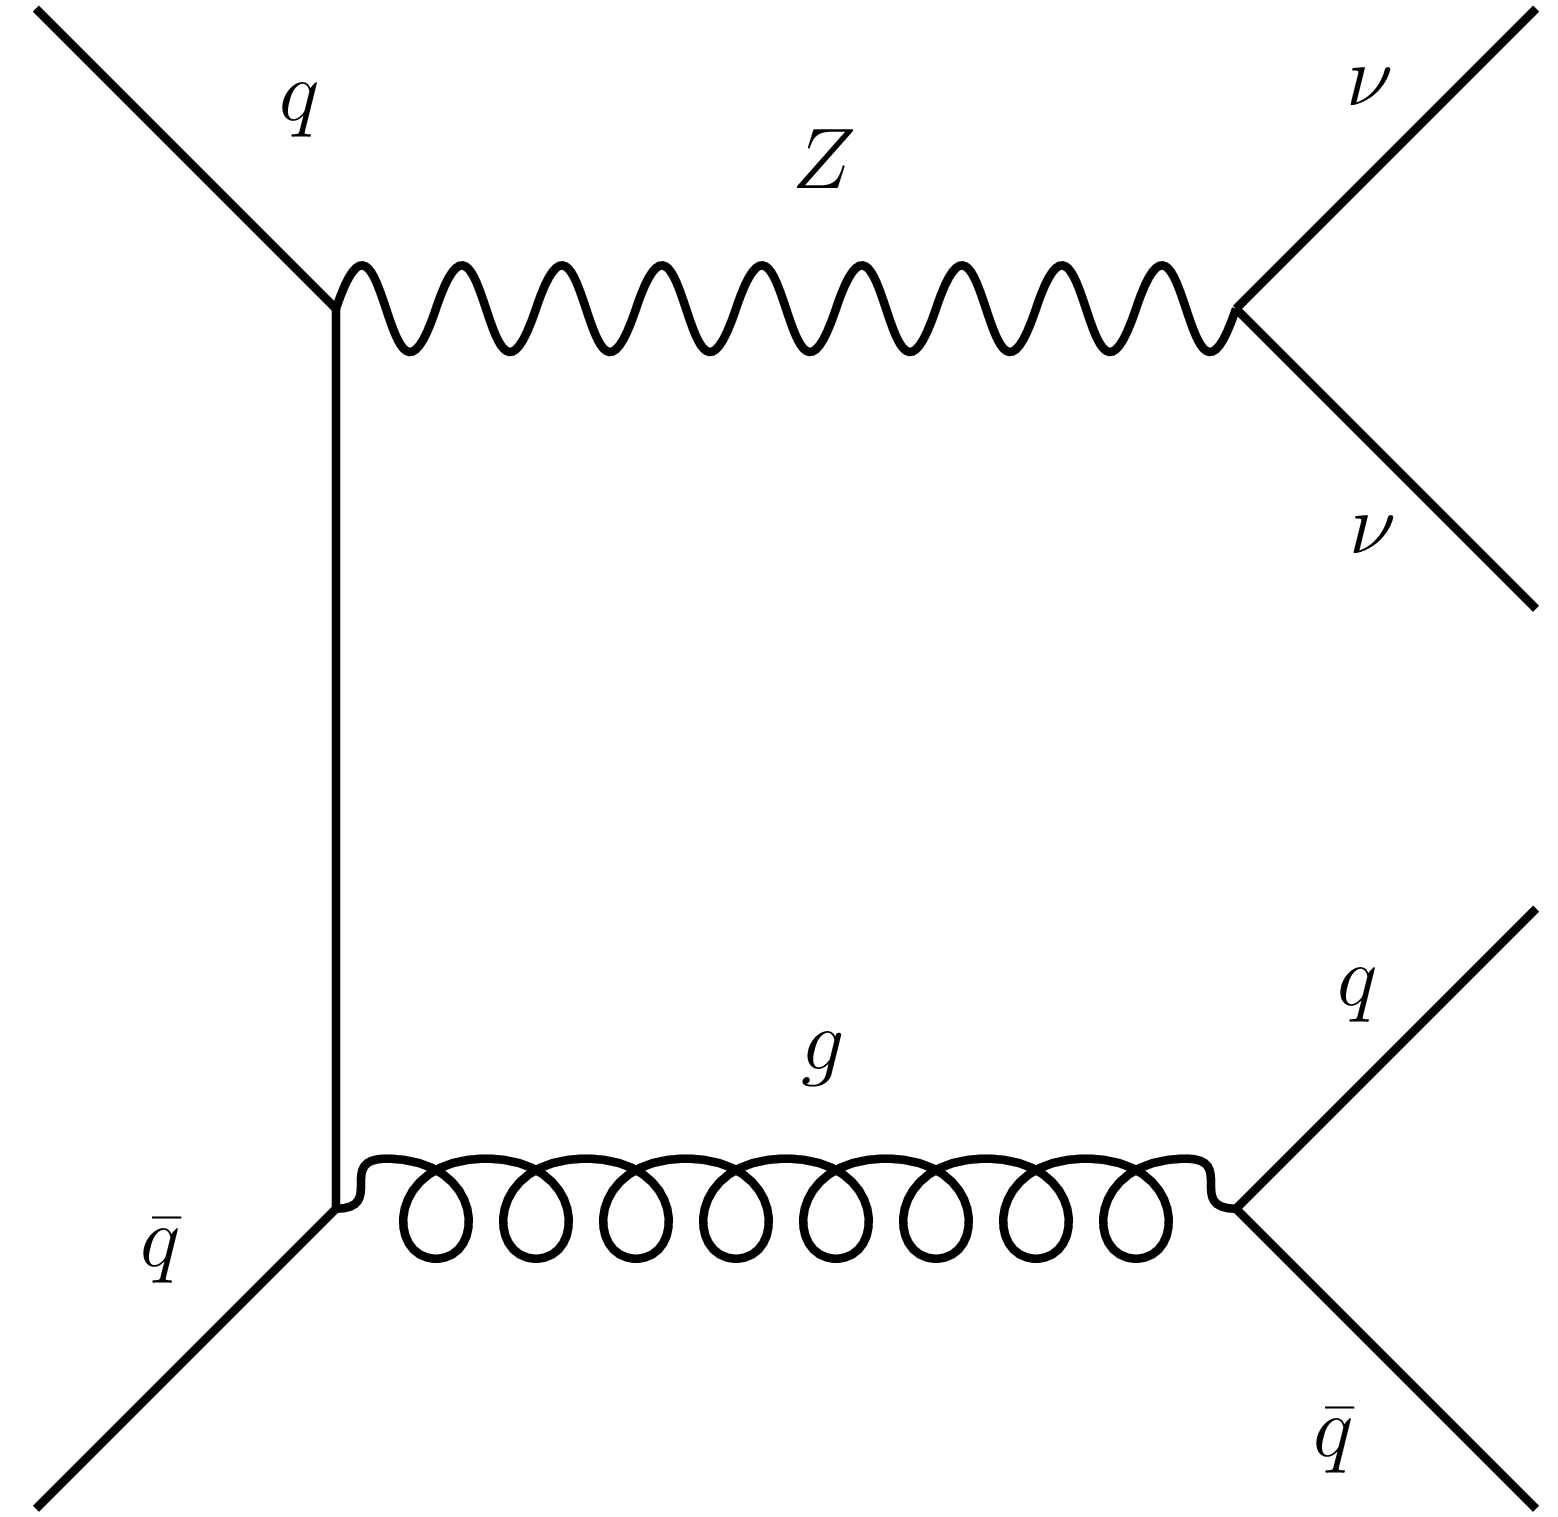
\includegraphics[width=0.3\linewidth]{Zvv.png}}
	~
	\subcaptionbox
	{$W$($l\nu$) + jets
		\label{fig:Bkg-Processes-fig2}}
	{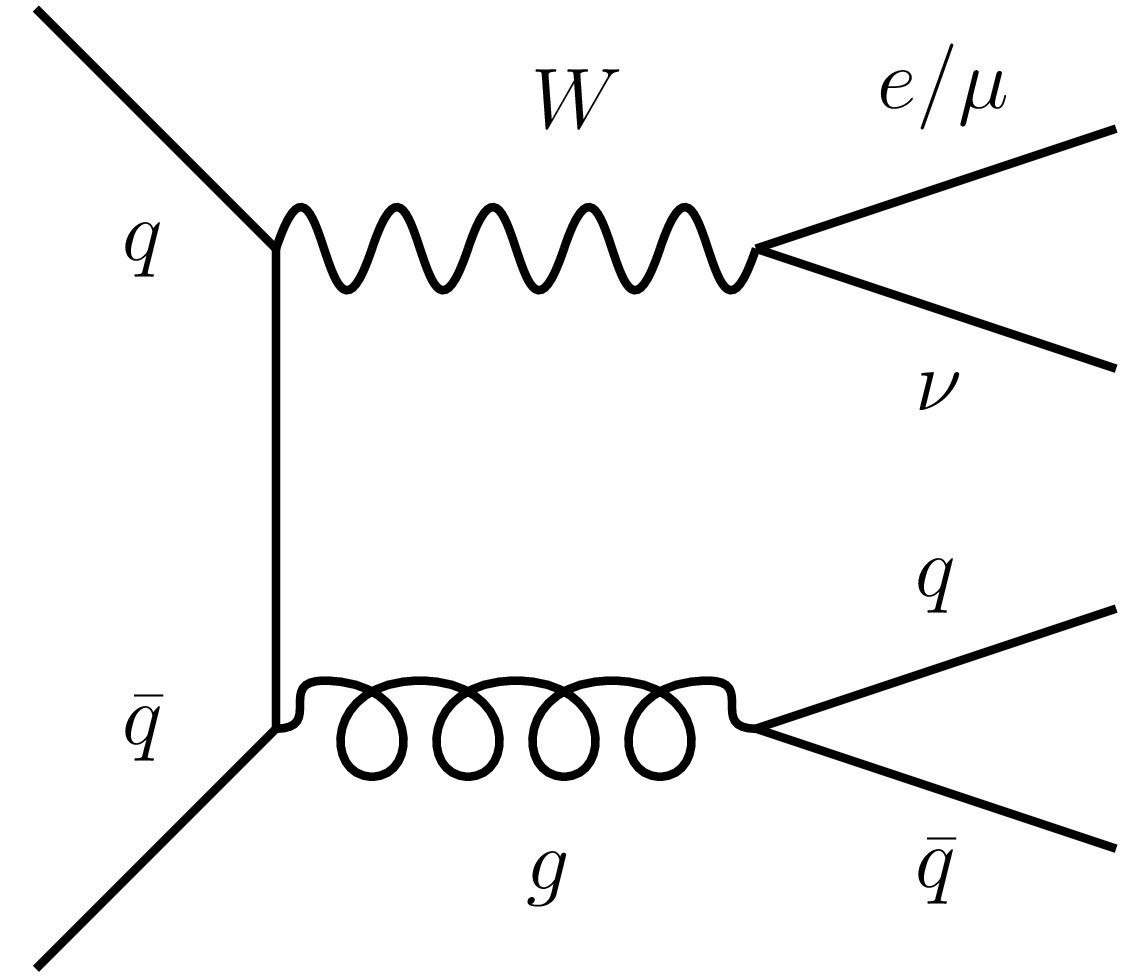
\includegraphics[width=0.3\linewidth]{Wlv.png}}
	~
	\subcaptionbox
	{$t\bar{t}$
		\label{fig:Bkg-Processes-fig3}}
	{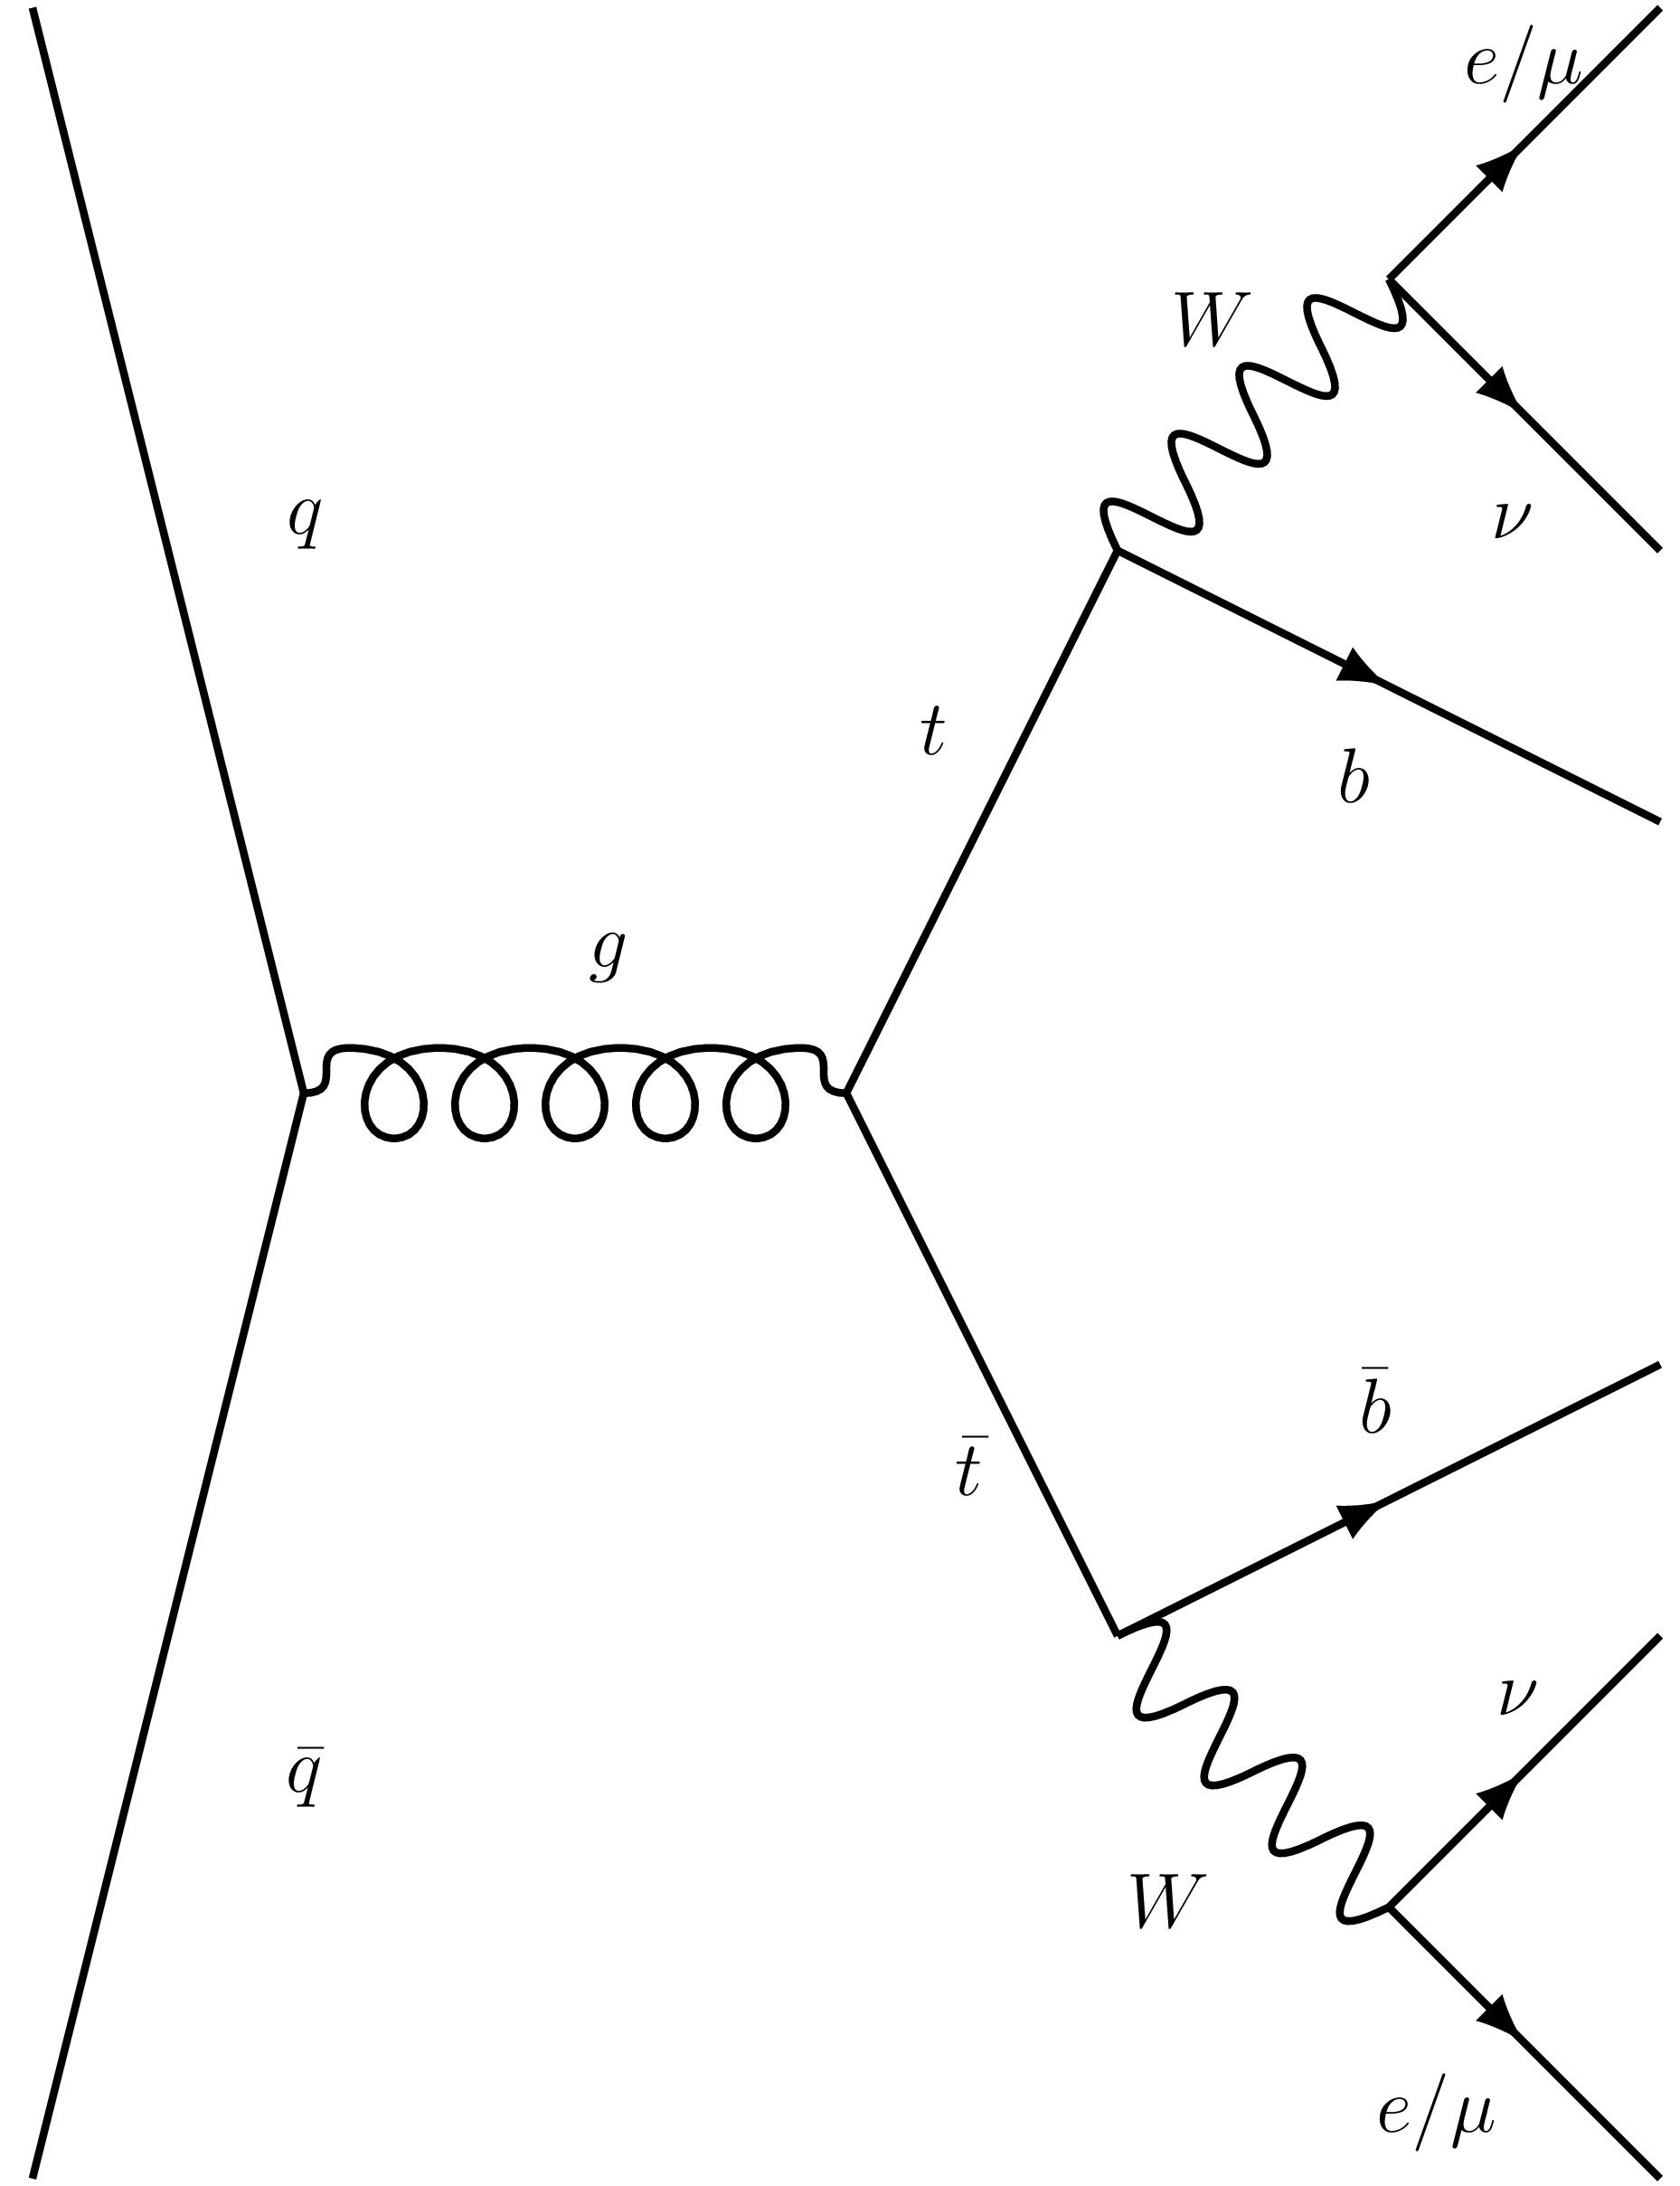
\includegraphics[width=0.3\linewidth]{ttbar.png}}
	\caption{The main background processes of the monoH analysis.}
	\label{fig:Bkg-Processes}
\end{figure}

\end{document}